\documentclass{article}
%% \usepackage{times}

\usepackage{float}
\usepackage{latexsym}
\usepackage{url}
\usepackage{hyperref}
\hypersetup{colorlinks=true}
\usepackage{enumitem,amssymb}
\usepackage{graphicx}
\graphicspath{ {./images/} }
\newlist{todolist}{itemize}{4}
\setlist[todolist]{label=$\square$}
\begin{document}

\begin{titlepage}
	\centering
    \vspace{3cm}
	{\scshape\Large Artificial Intelligence Assignment \par}
	\vspace{4cm}
	{\huge\bfseries\LARGE BLOCKS WORLD PROBLEM \par}
	\vspace{2cm}
	{\Large STUDENT: POP DIANA-\c{S}TEFANIA\par}
	\vspace{1cm}
	{\Large GROUP: C.EN. 2.2A\par}
	\vspace{1cm}
	{\Large YEAR: II\par}
	\vspace{1cm}
	\vfill
% Bottom of the page
\end{titlepage}

\begin{centering}
\vspace{1cm}
{\scshape\Large Technical report \par}
\end{centering}
\vspace{1.5cm}
% sections
\section{Problem statement}
A set of wooden blocks of various shapes and colors are sitting on a table. The goal is to build one or more vertical stacks of blocks. The catch is that only one block may be moved at a time: it may either be placed on the table or placed atop another block. Because of this, any blocks that are, at a given time, under another block cannot be moved. 
\\
\textbf{Initial state} : Given configuration of blocks and a set of block stacks.
\\
\textbf{Actions and transitions} : Move block from the top of one stack onto the table or onto the top of another stack.
\\
\textbf{Goal} : A given final configuration of the stacks of blocks.
\\


\section{Pseudocode}

Presented below are the algorithms used for defining the heuristics, for computing the resulted state after performing a certain action and for determining the possible actions:

%\begin{figure}[ht]
\begin{center}
\begin{tabbing}
\textbf{ACTIONS} ($state$) \\
\rhd$ Computes the possible actions to be taken in the current state and\\ returns their list$\\
1. \indent {\bf for} \=stack \textbf{in} \textit{state} {\bf do} \\
2. \indent\>{\bf for} \={other\_stack} \textbf{in} \textit{state} {\bf do} \\
3. \indent\>\>{\bf if}  \={other\_stack} != stack {\bf then} \\
4. \indent\>\>\>{\bf append} ({actions\_list}, (\=$state \rightarrow index(stack)$,  \\
5. \indent\>\>\>\>$state \rightarrow index(other\_stack)$)\\
6. \indent\>{\bf if}  \={\bf length}(stack) != 1 {\bf then} \\
7. \indent\>\>{\bf append} (actions\_list, ($state \rightarrow index(stack)$, \textbf{none}) \\
8. \indent \textbf{return} {actions\_list}\\
\\
\textbf{Note :} \textbf{none} (no stack) can be represented as anything\\
(for example ' '), except as a natural number (used to enumerate the stack indexes).
\end{tabbing}
\end{center}
%\end{figure}
\vspace{8cm}
\vfill

%\begin{figure}[ht]
\begin{center}
\begin{tabbing}
\textbf{RESULT} ($state$, $action$) \\
\rhd$ Computes the resulting state based on a certain action \\and the current state$\\
1. \indent $source\_stack \leftarrow action[0]$ \\
2. \indent $destination\_stack \leftarrow action[1]$\\
3. \indent $moved\_block \leftarrow$ last element in $state\_list[source\_stack]$\\
4. \indent \textbf{if  \= length}(\textit{state}[{source\_stack}]) != 1 \textbf{then}\\
5. \indent\>\textbf{for \=} $iterator \leftarrow 0, length(state[source\_stack]-1$ \textbf{do}\\
6. \indent\>\>\textbf{append}($new\_stack, state[source\_stack][iterator]$)\\
7. \indent\>\textbf{append}({state\_list, new\_stack})\\
8. \indent \textbf{if \=} {destination\_stack} != \textbf{none} \textbf{then}\\
9. \indent \>\textbf{remove}({state\_list, \textit{state}[destination\_stack]})\\
10. \indent \>\textbf{append}({state\_list, \textit{state}[destination\_stack] + (moved\_block)})\\
11. \indent\textbf{el\=se}\\
12. \indent\>\textbf{append}({state\_list, (moved\_block)})\\
13. \indent \textbf{remove}({state\_list, \textit{state}[source\_stack])}\\
14. \indent \textbf $state\_list \rightarrow \textbf{sort\_by}(\textbf{length}(stack))$\\
15. \indent \textbf{return} {state\_list}\\
\\
\textbf{Note :} \textbf{none} (no stack) can be represented as anything\\
(for example ' '), except as a natural number (used to enumerate the stack indexes).
\end{tabbing}
\end{center}
%\end{figure}

%\begin{figure}[ht]
\begin{center}
\begin{tabbing}
\textbf{H1} ($node$) \\
\rhd$ Checks whether a block is in the right place and returns \\the number of blocks out of place $\\
1. \indent $sum \leftarrow 0$ \\
2. \indent \textbf{for\=} stack \textbf{in} $node \rightarrow state$ \textbf{do} \\
3. \indent \>\textbf{for\=} block \textbf{in} stack \textbf{do} \\
4. \indent \>\>\textbf{for\=} {other\_stack} \textbf{in} goal \textbf{do} \\
5. \indent \>\>\>\textbf{if \=} block \textbf{in} {other\_stack} \textbf{then}\\
6. \indent \>\>\>\>$block\_position\leftarrow stack\rightarrow index(block)$\\
7. \indent \>\>\>\>$other\_position\leftarrow other\_stack\rightarrow index(block)$\\
8. \indent \>\>\>\>\textbf{if \=} {block\_position} == 0 \textbf{or} {other\_position == 0 } \\ 
9. \>\>\>\>\textbf{and} {block\_position} != {other\_position}\\  10.\>\>\>\>\textbf{or} stack[{block\_position}-1] != stack[{other\_position}-1] \textbf{then}\\
11.\>\>\>\>\>$sum\leftarrow sum + 1$\\
12.\>\>\>\>\>\textbf{break}\\
13. \indent \textbf{return} sum\\
\vspace{8cm}
\vfill

\end{tabbing}
\end{center}
%\end{figure}

%\begin{figure}[ht]
\begin{center}
\begin{tabbing}
\textbf{H2} ($node$) \\
\rhd$ Counts the number of moves than need to be done in order \\ for every block to reach its correct place $\\
1. \indent $sum \leftarrow 0$ \\
2. \indent\textbf{for \=} stack \textbf{in} $node\rightarrow state$ \textbf{do}\\
3. \indent\>\textbf{for \=} {other\_stack} \textbf{in} goal \textbf{do}\\
4. \indent \>\>\textbf{if \=} stack[0] \textbf{in} goal \textbf{then}\\
5. \indent \>\>\>$goal\_stack\leftarrow other\_stack$\\
6. \indent \>\>\>\textbf{break}\\
7. \indent\>\textbf{for \=} block \textbf{in} stack \textbf{do}\\
8. \indent\>\>$block\_position\leftarrow stack\rightarrow index(block)$\\
9. \indent\>\>\textbf{if \=} block \textbf{in} {goal\_stack} \textbf{then}\\
10. \indent\>\>\>\textbf{if \=} $block\_position == goal\_stack\rightarrow index(block)$ \textbf{then}\\
11. \indent\>\>\>\>\textbf{continue}\\
12. \indent\>\> $sum\leftarrow sum + \textbf{length}(stack) - block\_position$\\
13. \indent\>\>\textbf{for \=} $iterator\leftarrow block\_position,\textbf{length}(stack)$ \textbf{do}\\
14. \indent\>\>\> $stack\_block\leftarrow stack[iterator]$\\
15. \indent\>\>\> $stack\_position\leftarrow stack\rightarrow \textbf{index}(stack\_block)$\\
16. \indent\>\>\>\textbf{if \=} {stack\_position} != 0 \textbf{then}\\
17. \indent\>\>\>\>\textbf{for \=} {other\_stack} \textbf{in} goal \textbf{do}\\
18. \indent\>\>\>\>\>\textbf{if \=} {stack\_block} \textbf{in} {other\_stack} \textbf{then}\\
19. \indent\>\>\>\>\>\>$other\_position\leftarrow other\_stack\rightarrow \textbf{index}(stack\_block)$\\
20. \indent\>\>\>\>\>\>\textbf{if \=} {other\_position} != 0 \textbf{then}\\
21. \indent\>\>\>\>\>\>\>\textbf{for \=} $iterator\_2\leftarrow 0,stack\_position$ \textbf{do}\\
22. \indent\>\>\>\>\>\>\>\>$other\_block\leftarrow stack[iterator\_2]$\\
23. \indent\>\>\>\>\>\>\>\>\textbf{if \=} {other\_block} \textbf{in}
{other\_stack} \textbf{then}\\
24. \indent \>\>\>\>\>\>\>\>\>\textbf{if \=} $other\_stack\rightarrow \textbf{index}(other\_block)$\\ 25.\indent \>\>\>\>\>\>\>\>\>$< other\_position$ \textbf{then}\\
26. \indent \>\>\>\>\>\>\>\>\>\>$sum\leftarrow sum + 1$\\
27. \indent \>\>\>\>\>\>\>\>\>\>\textbf{break}\\
28. \indent \textbf{return} sum\\

\end{tabbing}
\end{center}
%\end{figure}

\section{Application design}

    \subsection{\textbf{Architectural overview :}}
    \vspace{0.5cm}
  
    The application is structured in 5 modules : \textbf{main.py}, \textbf{problem.py},\\
    \textbf{blocks\_world.py}, \textbf{random\_state\_generator.py}, and \textbf{search.py}.
    
    The \textbf{problem.py} module contains the class \textbf{BlocksWorld} used to define the Blocks World problem, whereas \textbf{blocks\_world.py} is used to extend the class and implement problem heuristics.
    
    The module \textbf{random\_state\_generator.py} is used to generate a random state according to a number of blocks given.
    
    A state is represented as a \textit{"tuple of tuples"}, where each tuple contained by the main tuple represents a stack of blocks and their first element represents the base block.
    
    \textbf{Example:} The state from \textit{Figure 1} would be represented as \\
    \textbf{state = ((0, 1, 4 , 6 , 3, 2), (7, 5))}
    
    The module \textbf{search.py} is used for implementing the search algorithms \\ (A* and recursive best-first search) and it closely follows the \textbf{AIMA framework.}
    
    \begin{figure}[t]
    \caption{A random configuration for 8 blocks}
    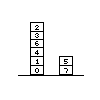
\includegraphics[width=6cm]{blocks}
    \centering
    \end{figure}
    
\subsection{\textbf{Input specification}}
The application will run using the \tetbf{main.py} module, and will ask the user to input a natural (non-zero) number which represents the number of blocks for the blocks world problem.
Then, there will be generated a random n-blocks world problem for which both searchers (A* and recursive best-first search) will be tested.

\subsection{\textbf{Output specification}}
There were made 10 tests using non-trivial input, the results being written in the files \textbf{output1.txt - output10.txt.}\\
The output presents a randomly generated initial and goal state for which the searchers are tested, and both solutions to the problem found by the searchers.\\
A solution represents the solution path (sequence of states) of the problem with the actions that lead to their specific states.\\
\\
\textbf{Example :} Action (1, 2) - move top block from stack 1 to stack 2 

\vfill



\begin{thebibliography}{9}
\label{sec_ref}

\bibitem{Blocks World problem}
\url{https://en.wikipedia.org/wiki/Blocks_world}
 \emph {Blocks World problem}.
 
 \bibitem{Random number generator}
\url{https://docs.python.org/3/library/random.html}
\emph {\\Random numbers generator}.
 
 \bibitem{Blocks World heuristics}
\url{http://www.d.umn.edu/~kvanhorn/cs2511/discussions/heuristics.html}\\
\url{https://www.d.umn.edu/~gshute/cs2511/projects/Java/assignment6/blocks/blocks.xhtml}
\emph{Blocks World heuristics}

\bibitem{AIMA python code}
\url{https://github.com/aimacode/aima-python}
 \emph {\\AIMA problem framework python}.

\bibitem{latex}
\LaTeX project site,
\url{http://latex-project.org/}

\end{thebibliography}



\end{document}



